\documentclass[../document.tex]{subfiles}
\begin{document}\label{ssec:time}
	
We first present execution time measurements for each benchmark, starting with the Cyclic Redundancy Check {\tt crc} benchmark which represents the Combinational Logic dwarf.

\newcommand{\plotwidth}{0.24\textwidth}
%\begin{figure*}[t]
%	\centering
%	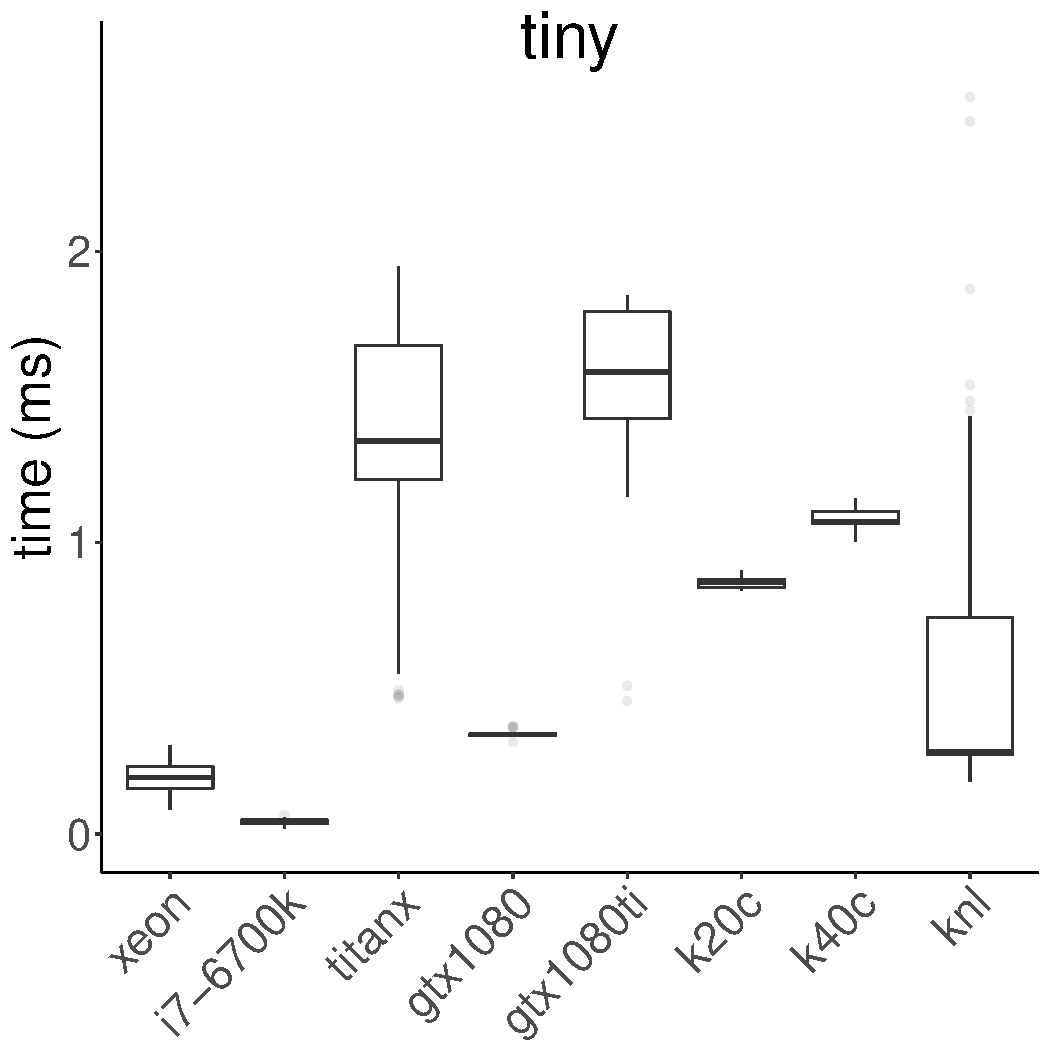
\includegraphics[width=\plotwidth]{figures/time-results/generate_crc_tiny_boxplot_knl-1}
%	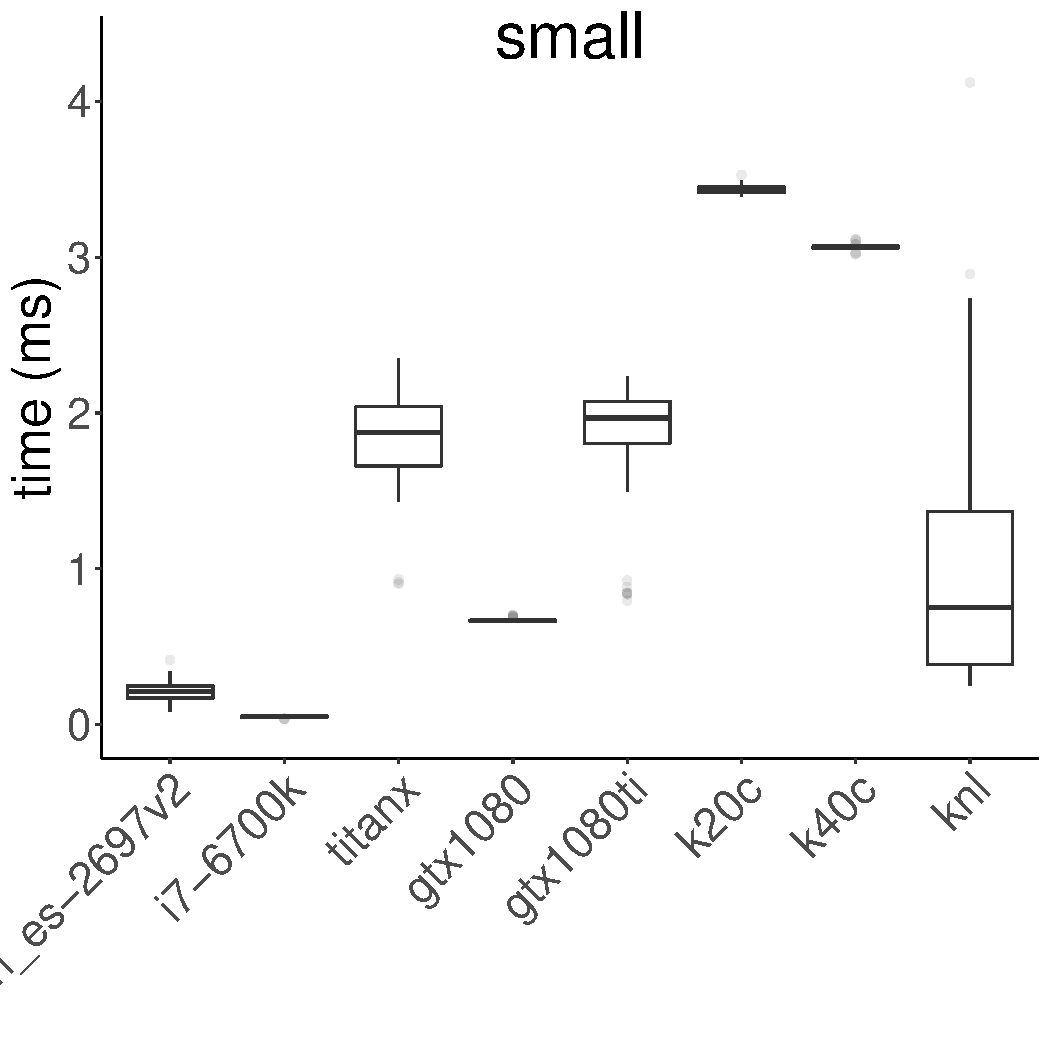
\includegraphics[width=\plotwidth]{figures/time-results/generate_crc_small_boxplot_knl-1}
%	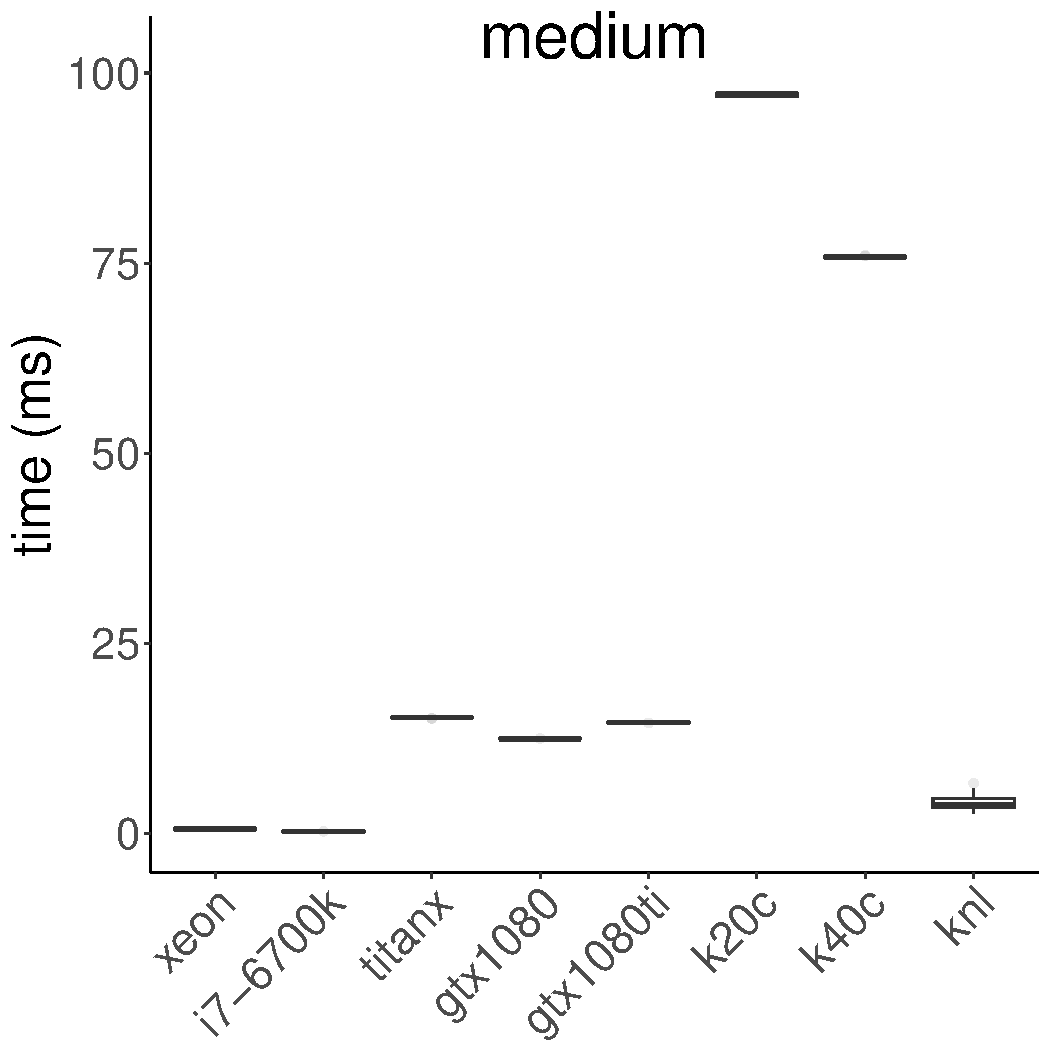
\includegraphics[width=\plotwidth]{figures/time-results/generate_crc_medium_boxplot_knl-1}
%	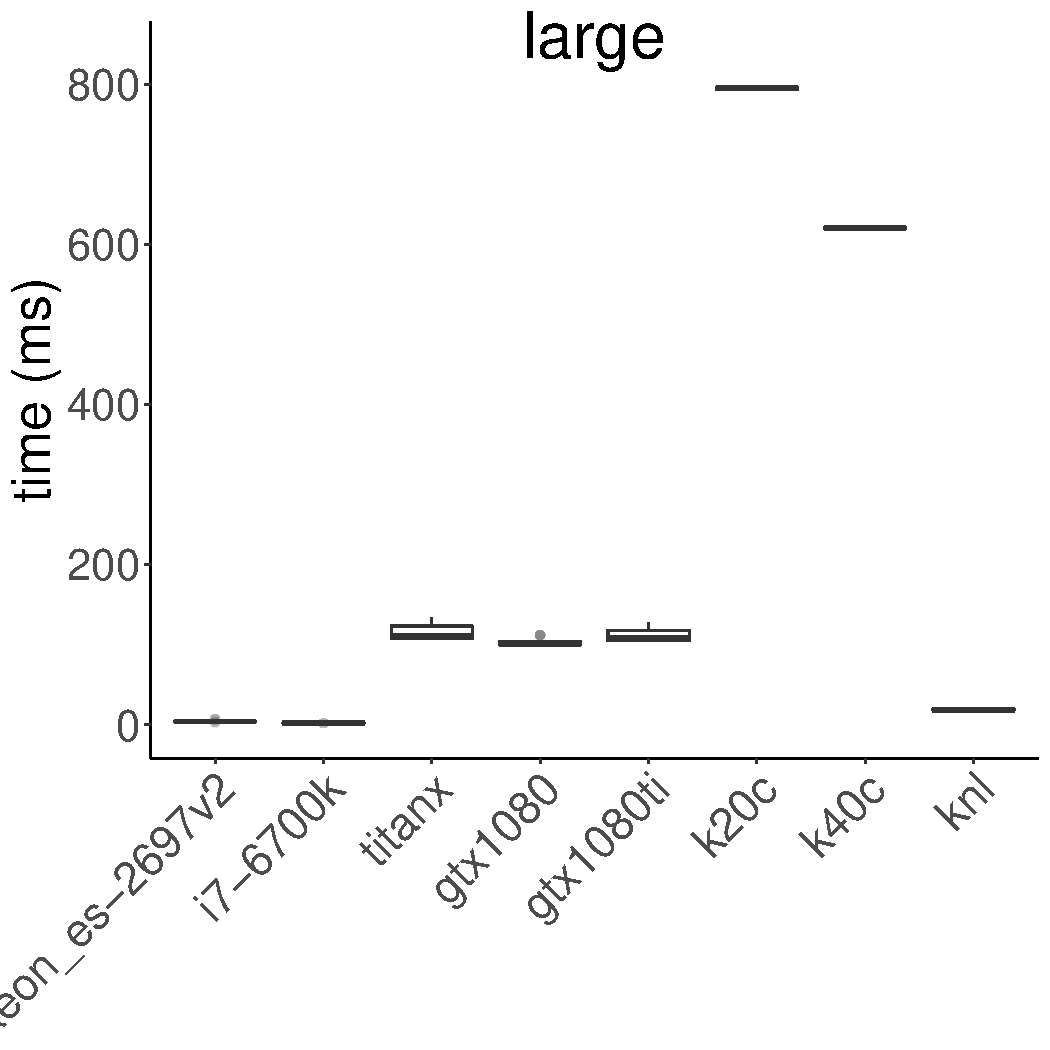
\includegraphics[width=\plotwidth]{figures/time-results/generate_crc_large_boxplot_knl-1}
%	\caption{Kernel execution times for the {\bf crc} benchmark on different hardware platforms, including KNL}
%	\label{fig:time-crc}
%\end{figure*}

\begin{figure*}[t]
	\centering
	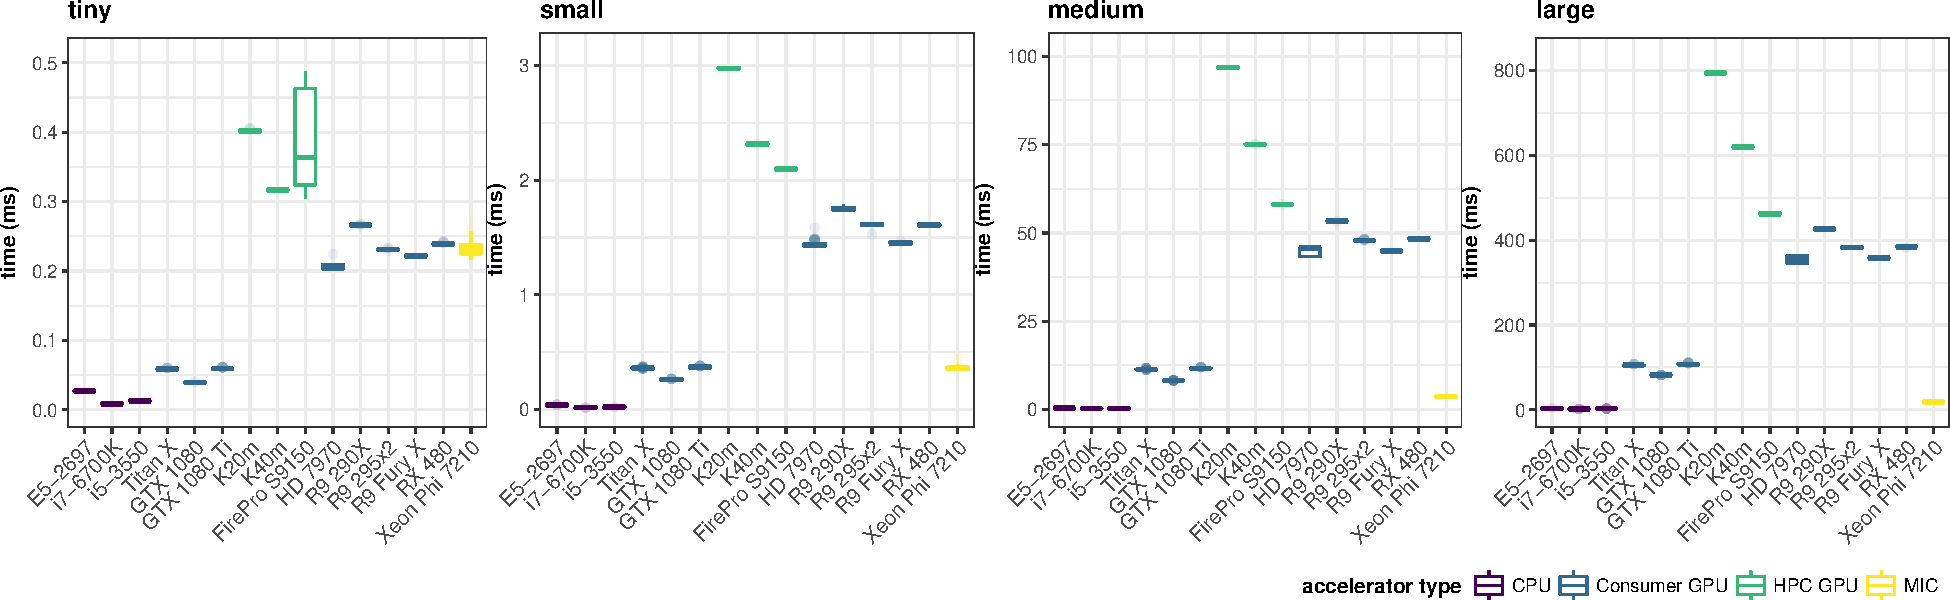
\includegraphics[width=\textwidth,keepaspectratio]{figures/new-time-results/generate_crc_row_bandwplot}
	\caption{Kernel execution times for the {\bf crc} benchmark on different hardware platforms}
	\label{fig:time-crc}
\end{figure*}



Figure~\ref{fig:time-crc} shows the execution times for the {\tt crc} benchmark over 50 iterations on each of the target architectures, including the KNL.
The results have been coloured according to accelerator type: red for CPU devices, green for consumer GPUs, blue for HPC GPUs, and purple for the KNL MIC.
Execution times are lowest on CPU-type architectures, probably due to the low floating-point intensity of the CRC computation~\cite[Ch. 6]{joshi2016thesis}.
Excluding {\tt crc}, all the other benchmarks perform best on GPU type accelerators; furthermore, the performance on the KNL is poor due to the lack of support for wide vector registers in Intel's OpenCL SDK.
We therefore omit results for KNL for the remaining benchmarks.

\todo{We could examine the kiviat diagrams to see if they have high memory address entropy -- or high memory overhead which contributes to the why some benchmarks see a wide variation while others experience only a little, is this the major cause in variation?}
\todo{What are the major motivations for including this results section? We should conclude with these motivations and what has been shown accordingly}

Figures~\ref{fig:time} and~\ref{fig:time2} shows the distribution of kernel execution times for the remaining benchmarks.
Each benchmark corresponds to a particular dwarf: 
Figure~\ref{fig:time}a ({\tt kmeans}) represents the MapReduce dwarf,
Figure~\ref{fig:time}b ({\tt lud}) represents the Dense Linear Algebra dwarf,
Figure~\ref{fig:time}c ({\tt csr}) represents Sparse Linear Algebra, 
Figure~\ref{fig:time}d ({\tt dwt}) and Figure~\ref{fig:time}e ({\tt fft}) represent Spectral Methods,
Figure~\ref{fig:time2}a ({\tt srad}) represents the Structured Grid dwarf and Figure~\ref{fig:time2}b ({\tt nw}) represents Dynamic Programming.

Finally, Figure~\ref{fig:time3} presents results for the 3 applications with restricted problem sizes and only one problem size is shown.
The N-body Methods dwarf is represented by ({\tt gem}) and the results are shown in Figure~\ref{fig:time3}a, the Backtrack \& Branch and Bound dwarf is represented by the ({\tt nqueens}) application in Figure~\ref{fig:time3}b and ({\tt hmm}) results in Figure~\ref{fig:time3}c represent the Graphical Models dwarf.


\begin{figure*}
    \centering
    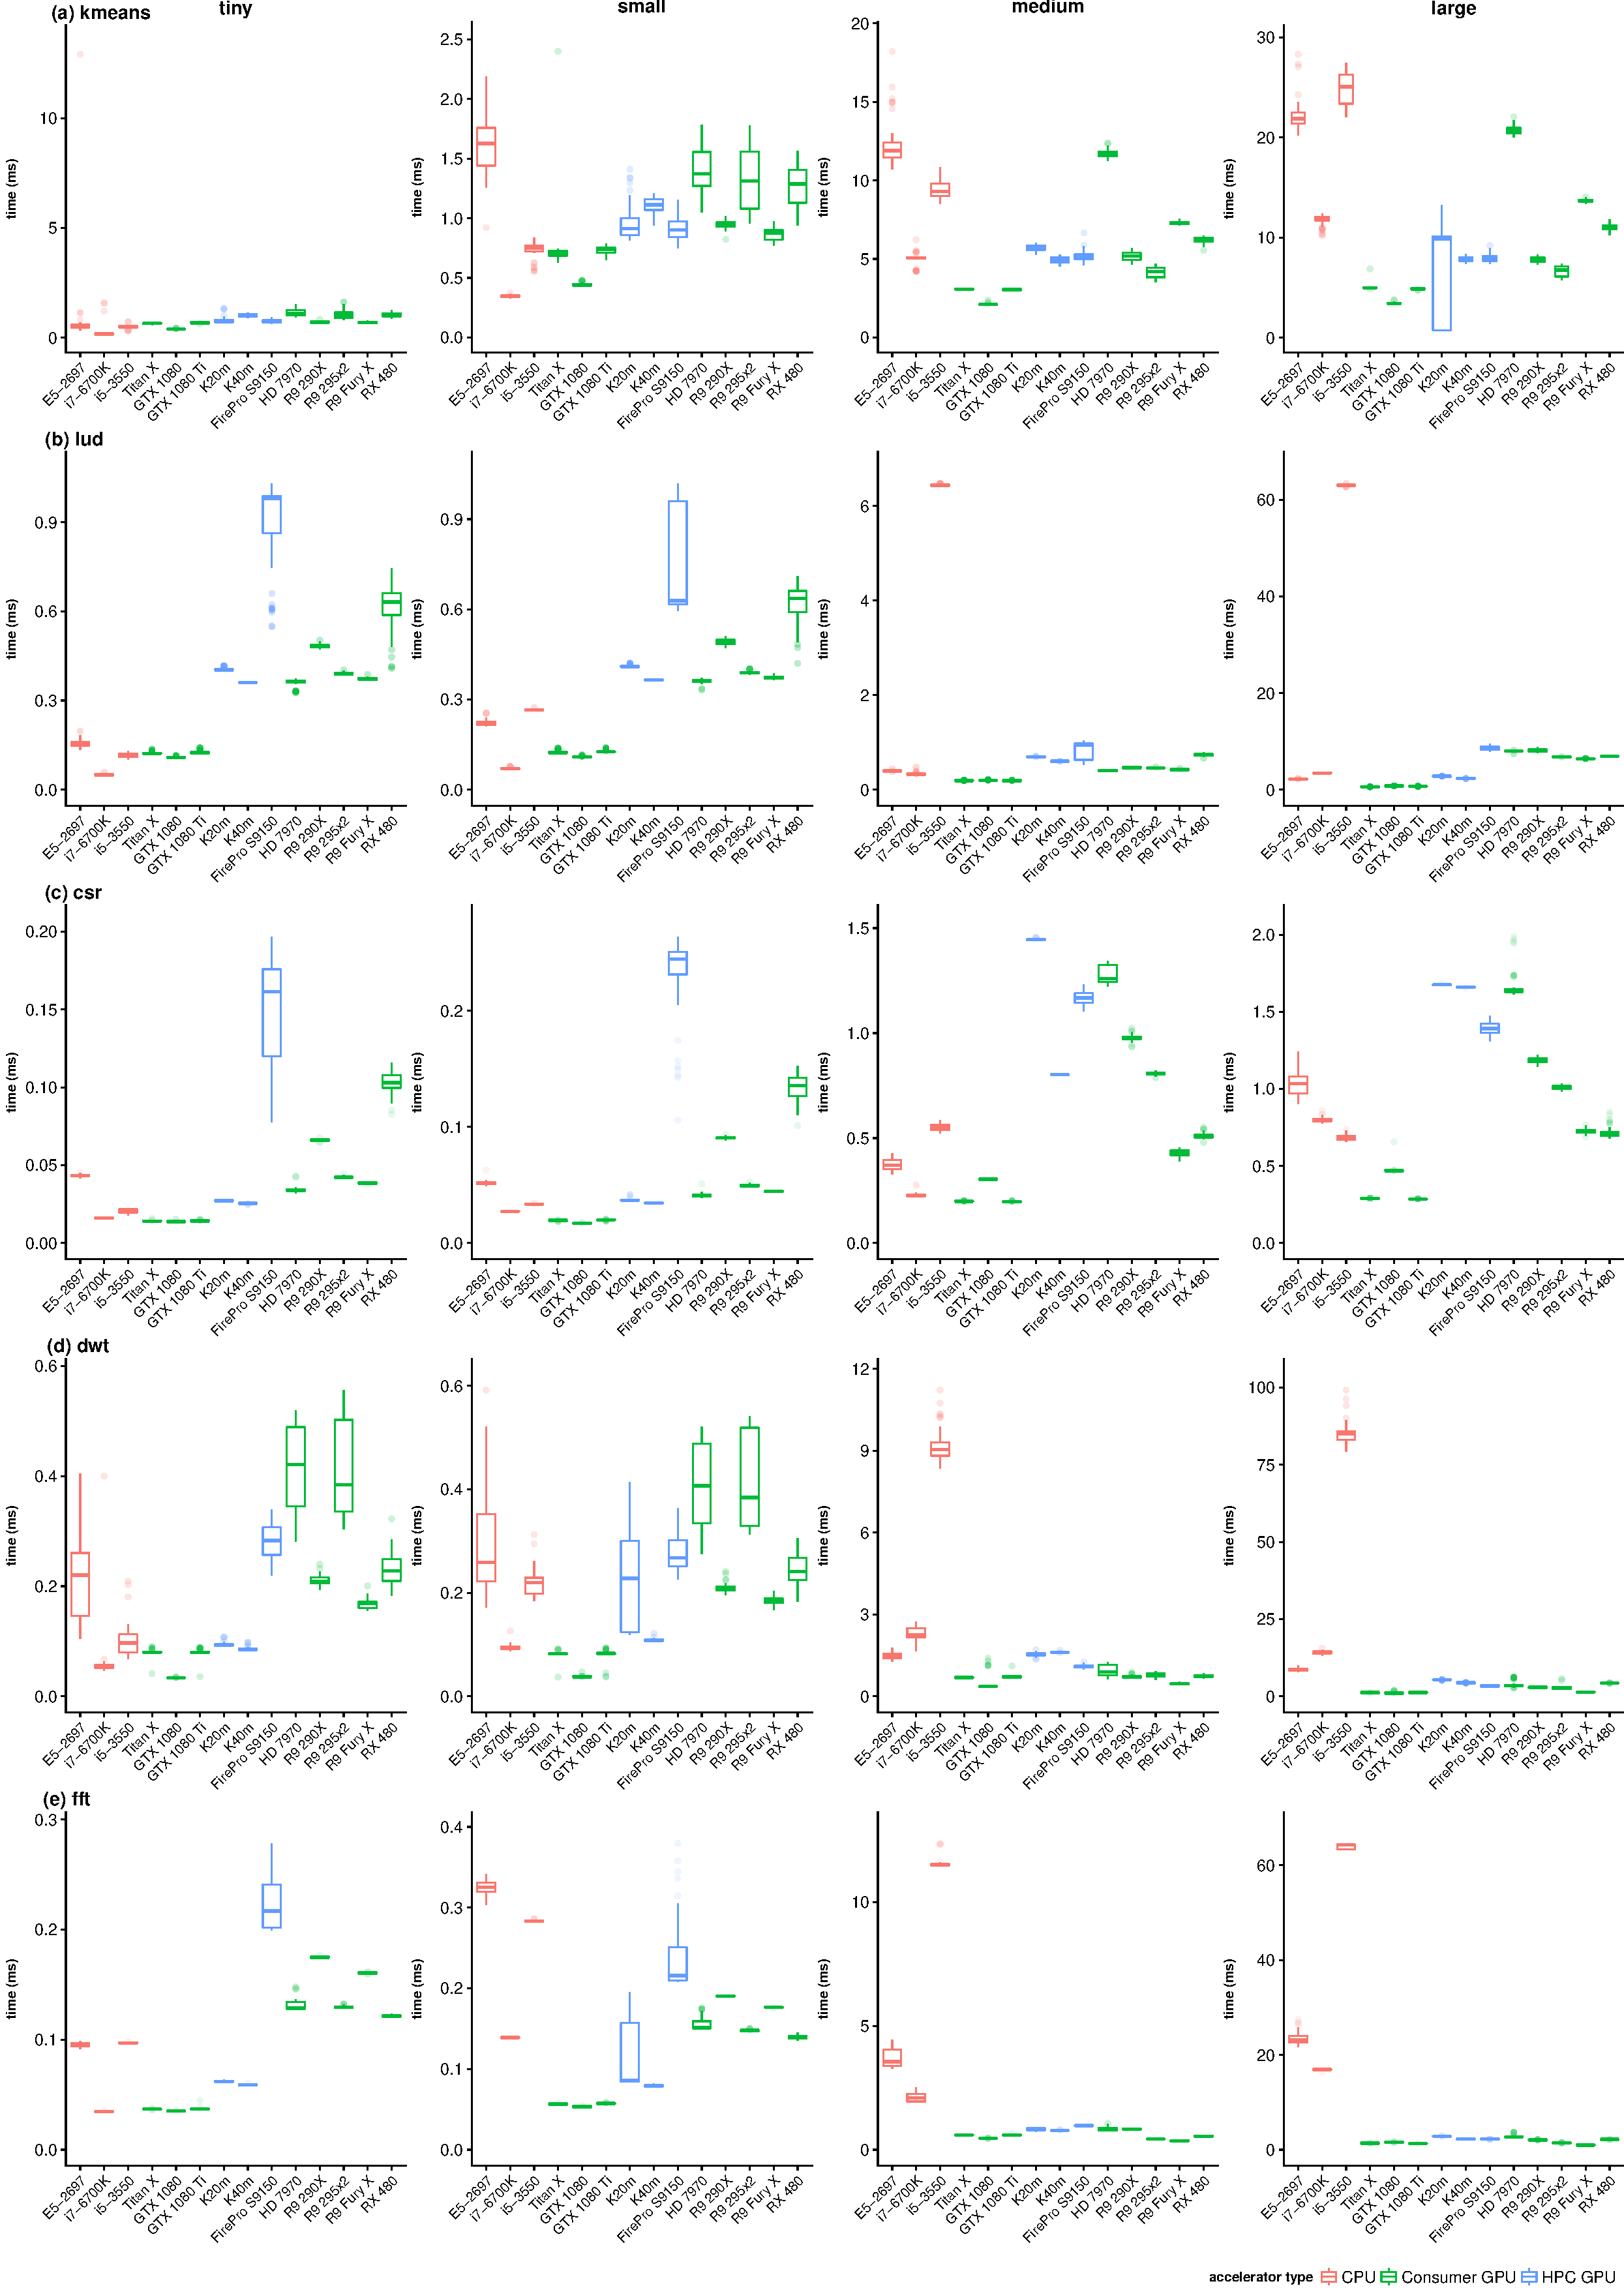
\includegraphics[width=.9\textwidth,keepaspectratio]{figures/new-time-results/generate_main_4x5_bandwplot}
    \caption{Benchmark kernel execution times on different hardware platforms}
    \label{fig:time}
\end{figure*}

\begin{figure*}[t]
    \centering
    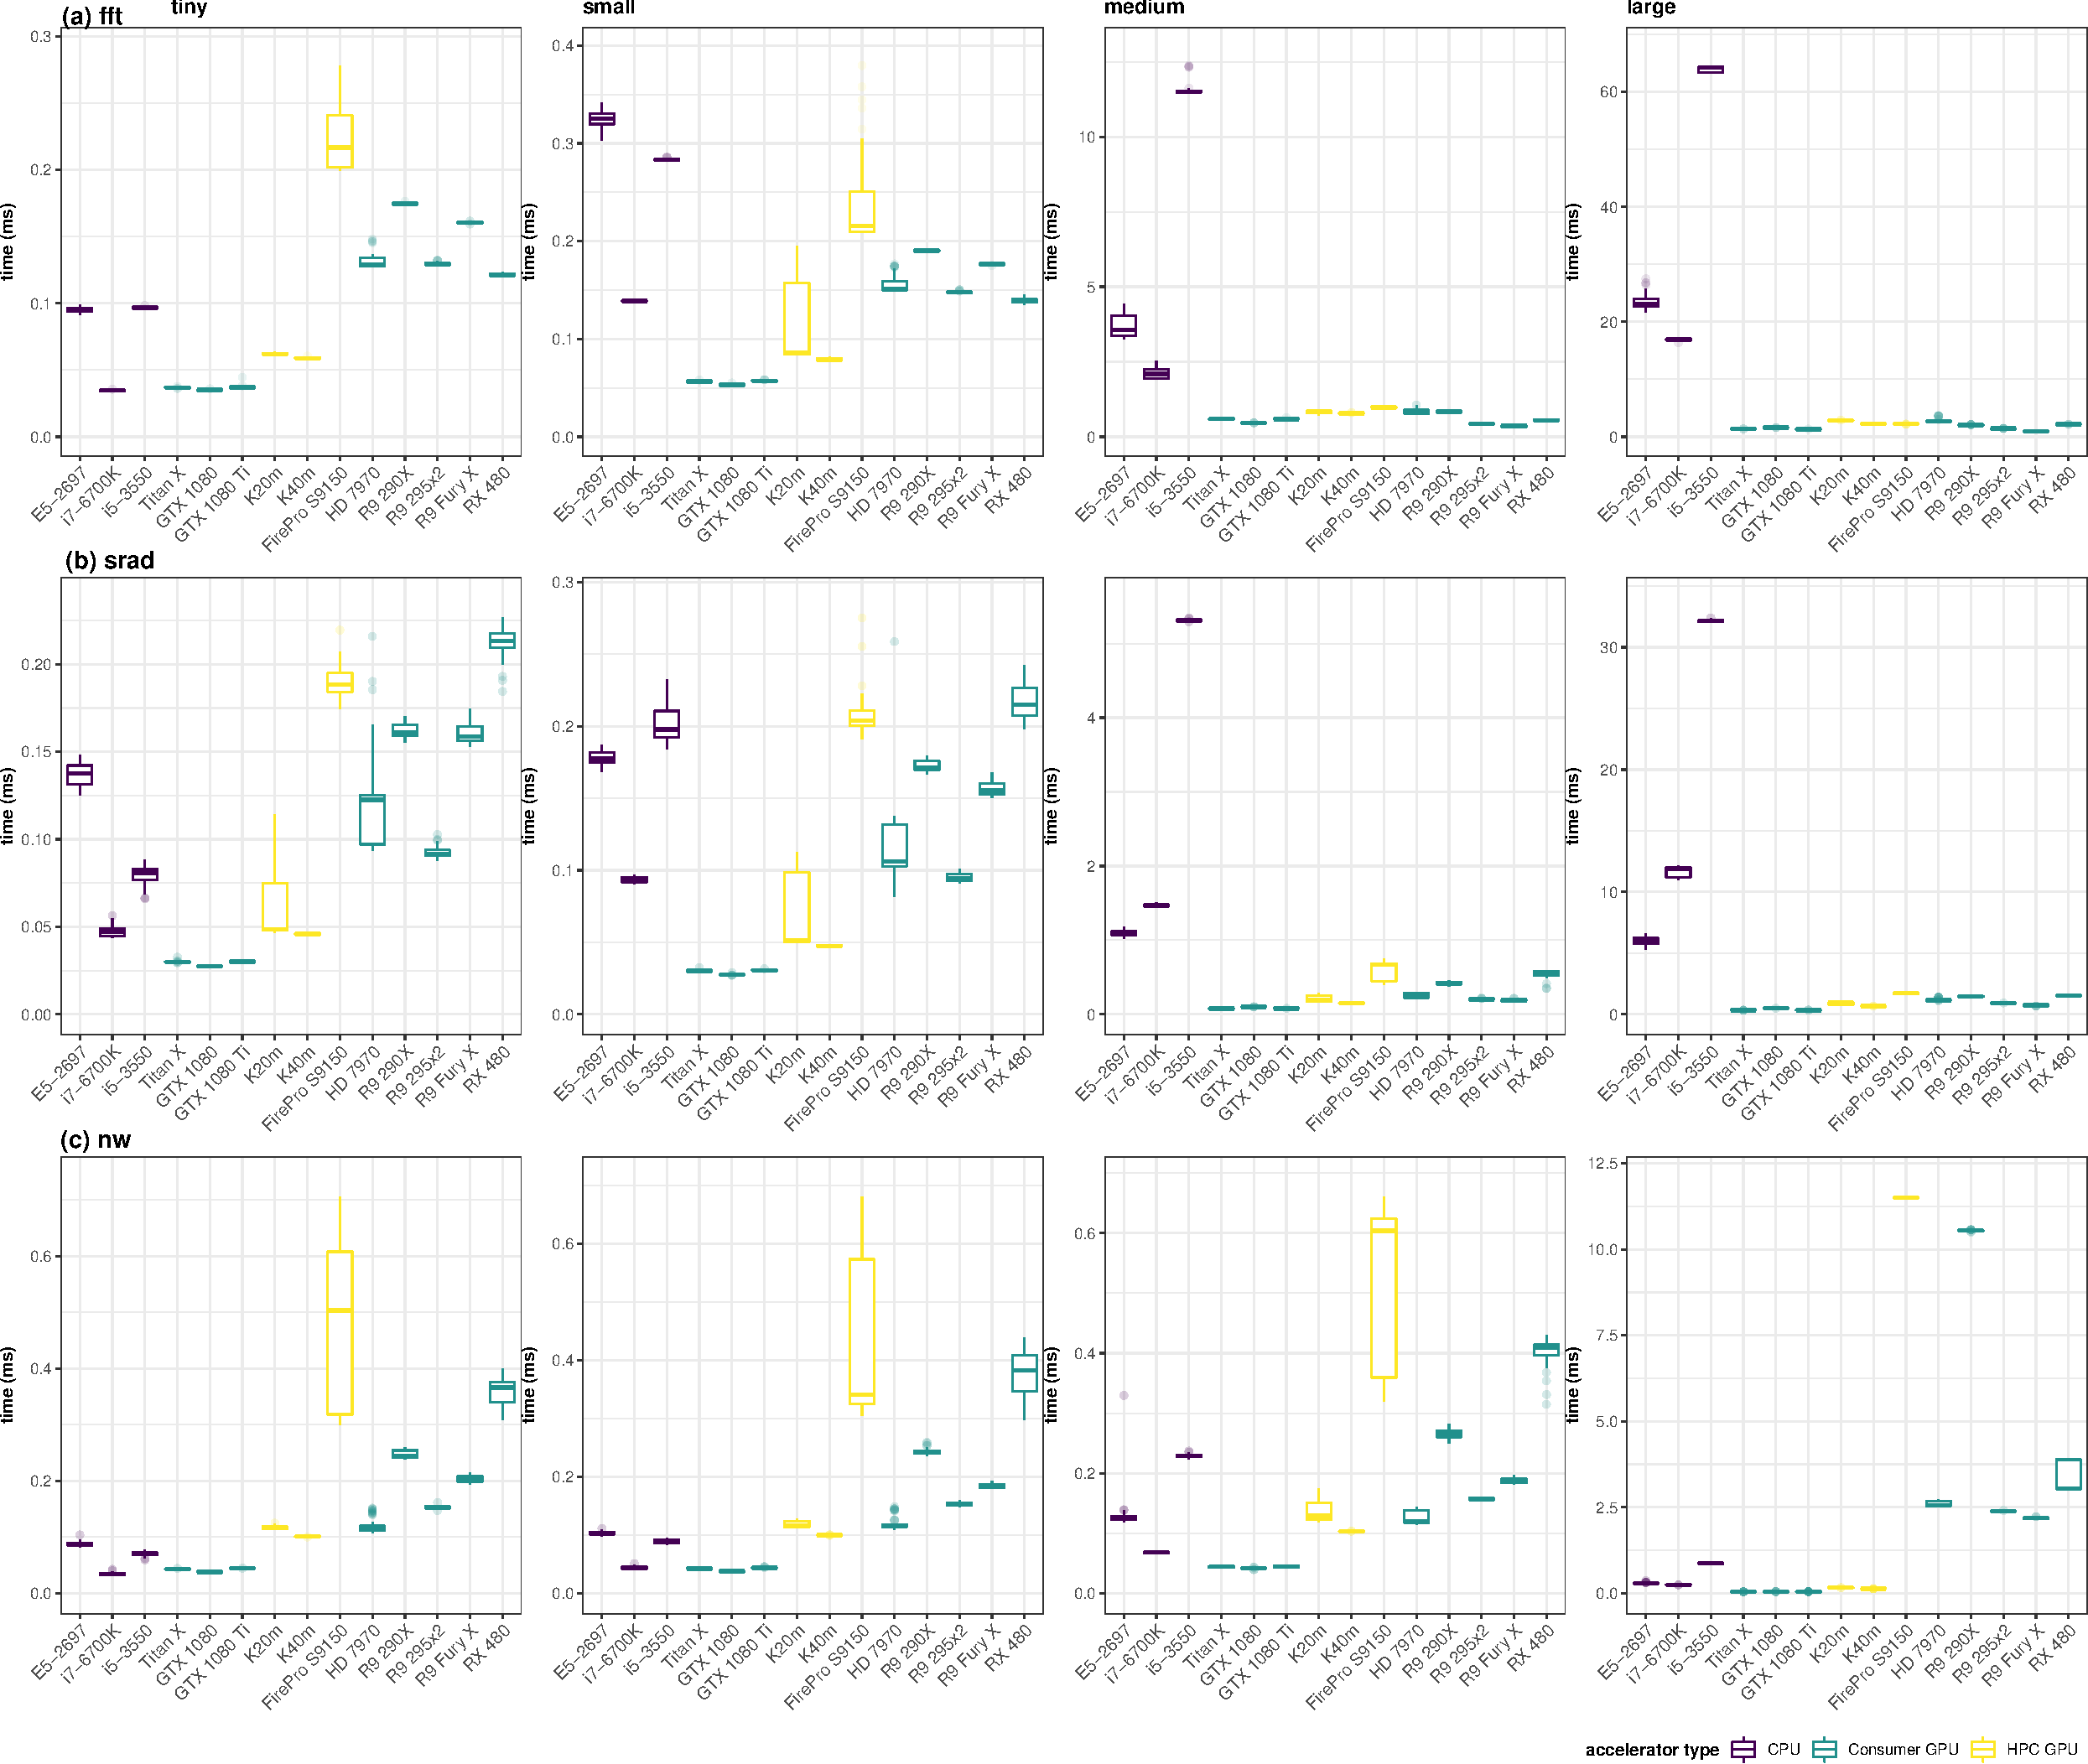
\includegraphics[width=\textwidth,keepaspectratio]{figures/new-time-results/generate_main_4x2_bandwplot}
    \caption{Benchmark kernel execution times on different hardware platforms (continued)}
    \label{fig:time2}
\end{figure*}

\begin{figure*}
    \centering
    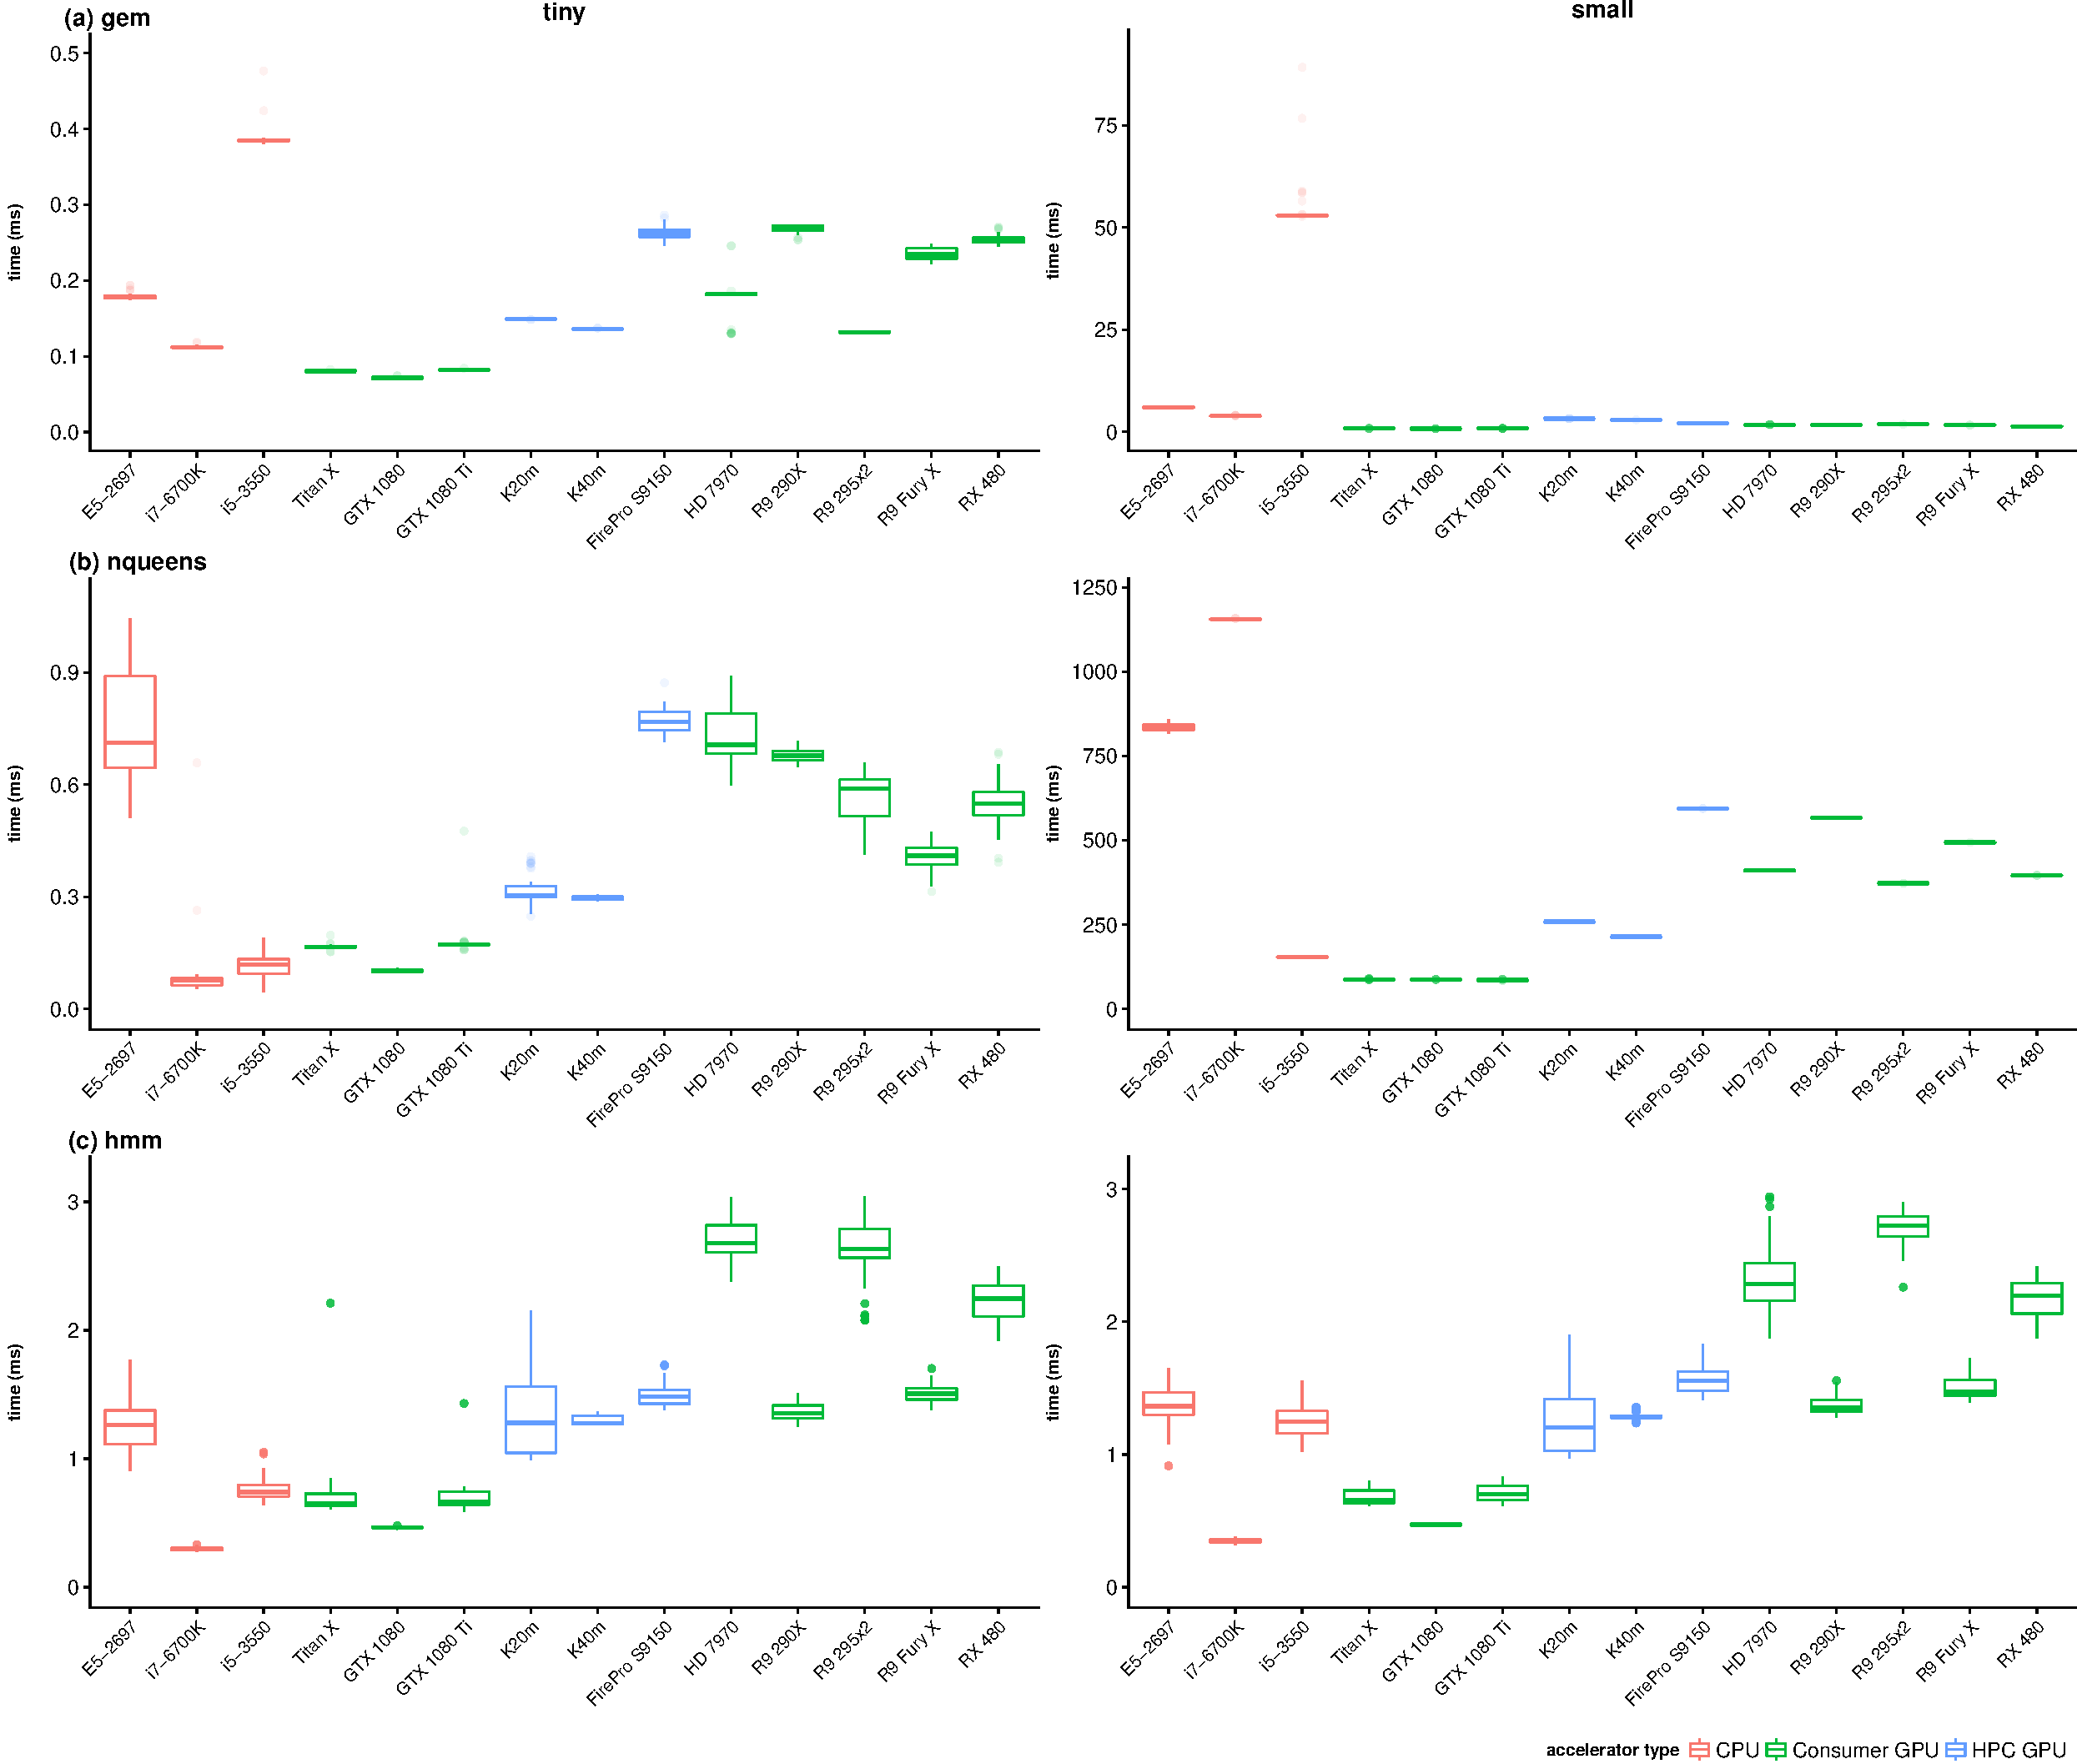
\includegraphics[width=\textwidth,keepaspectratio]{figures/new-time-results/generate_main_2x3_bandwplot}
    \caption{Smaller Benchmark kernel execution times on different hardware platforms}
    \label{fig:time3}
\end{figure*}


Examining the transition from tiny to large problem sizes (from left to right) in Figure~\ref{fig:time2}a shows the performance gap between CPU and GPU architectures widening for {\tt srad} -- indicating codes representative of structured grid dwarfs are well suited to GPUs.

In contrast, Figure~\ref{fig:time2}b shows Dynamic Programming problems have performance results tied to micro-architecture or OpenCL runtime support that are ill-classified by solely examining accelerator type.
For instance, the Intel CPUs and NVIDIA GPUs experience comparably over all problem sizes, whereas all AMD GPUs experience worst performance as size increases.

It isn't until many problem sizes are considered that these broader trends are discovered.

For most benchmarks, the variance in execution times is much greater devices with a lower clock frequency regardless of accelerator type.
While execution time increases with problem size for all benchmarks and platforms, the modern GPUs (Titan X, GTX1080, GTX1080Ti, R9 Fury X and RX 480) performed relatively better for large problem sizes, possibly due to their greater second-level cache size compared to the other platforms.
A notable exception is {\tt k-means} for which CPU execution times were comparable to GPU, which reflects the relatively low ratio of floating point to memory operations in the benchmark.

Generally, the HPC GPUs are older and were constructed to alleviate global memory limitations amongst consumer GPUs of the time.
Global memory size is not listed in Table~\ref{tab:hardware} since all selected problem sizes fit within the global memory of all devices.
However, despite larger memory sizes the clock speed of all HPC GPUs is slower than all evaluated consumer GPUs and thus have the worst performance of all GPU devices.
Indeed, at best they offer comparable execution times to the consumer GPUs for larger sized {\tt lud}, {\tt dwt}, {\tt fft} and {\tt srad} applications, and are perform equally with consumer GPUs over tiny and small problem sizes for all results presented in Figure~\ref{fig:time3}.

A comparison between CPUs over different problem sizes indicates the importance of examining multiple sized problems.
Medium sized problems were designed to fit within the L3 cache of the i7-6700K system, and this conveniently also fits within the L3 cache of the Xeon E5-2697 v2.
However, the older i5-3550 CPU has a smaller L3 cache and experiences worse performance when moving from small to medium sized problems, and is shown in Figures~\ref{fig:time}b,~\ref{fig:time}d,~\ref{fig:time}e and ~\ref{fig:time2}a,

Increasing problem size also hinders the performance in certain circumstances for GPU devices.
For example, Figure~\ref{fig:time2}b shows a widening performance gap over each increase in problem size between AMD GPUs and the other devices.

A brief study around the similarities within a dwarf and the differences between them can be presented based on the presented runtime results.
Asanovi\'{c} et al.~\cite{asanovic2006landscape} state that applications from the Spectral Methods dwarf is Memory latency limited,indeed if we examine {\tt dwt} and {\tt fft} -- the applications which represent Spectral Methods -- in Figure~\ref{fig:time}d andFigure~\ref{fig:time}e respectively, we see that in the medium problem sizes the execution times match the higher memory latency of the L3 cache of CPU devices relative to the GPU counterparts.
The trend only increases with problem size, since the large sized problem shows the CPU devices frequently accessing main memory while the GPUs larger memory ensures a lower memory access latency.
It is expected if had we extended this study to an even larger problem size that would not fit on GPU global memory, much higher perfomance penalties would be experienced over GPU devices, since the PCI-E interconnect has a higher latency than a memory access to main memory from the CPU systems.

Furthermore, Asanovi\'{c}et al.~\cite{asanovic2006landscape} state that the Structured Grid dwarf is memory bandwidth limited, the application representative of Structured Grid is {\tt srad} and the results over the larger problem sizes in Figure~\ref{fig:time2}a show that GPUs experience lower execution times than CPUs, this conforms to the performance limit claim, GPU devices offer a higher bandwidth than a system interconnect.

\todo[inline]{The remaining applications could be examined in terms of dwarf}

\end{document}
